\documentclass[border=10pt]{standalone}
\usepackage[svgnames]{xcolor}
\usepackage{amsmath}
\usepackage{pgfplots}
\pgfplotsset{compat=newest}
\usepackage[sfdefault]{FiraSans}
\usepackage{FiraMono}
\renewcommand*\familydefault{\sfdefault}
\begin{document}
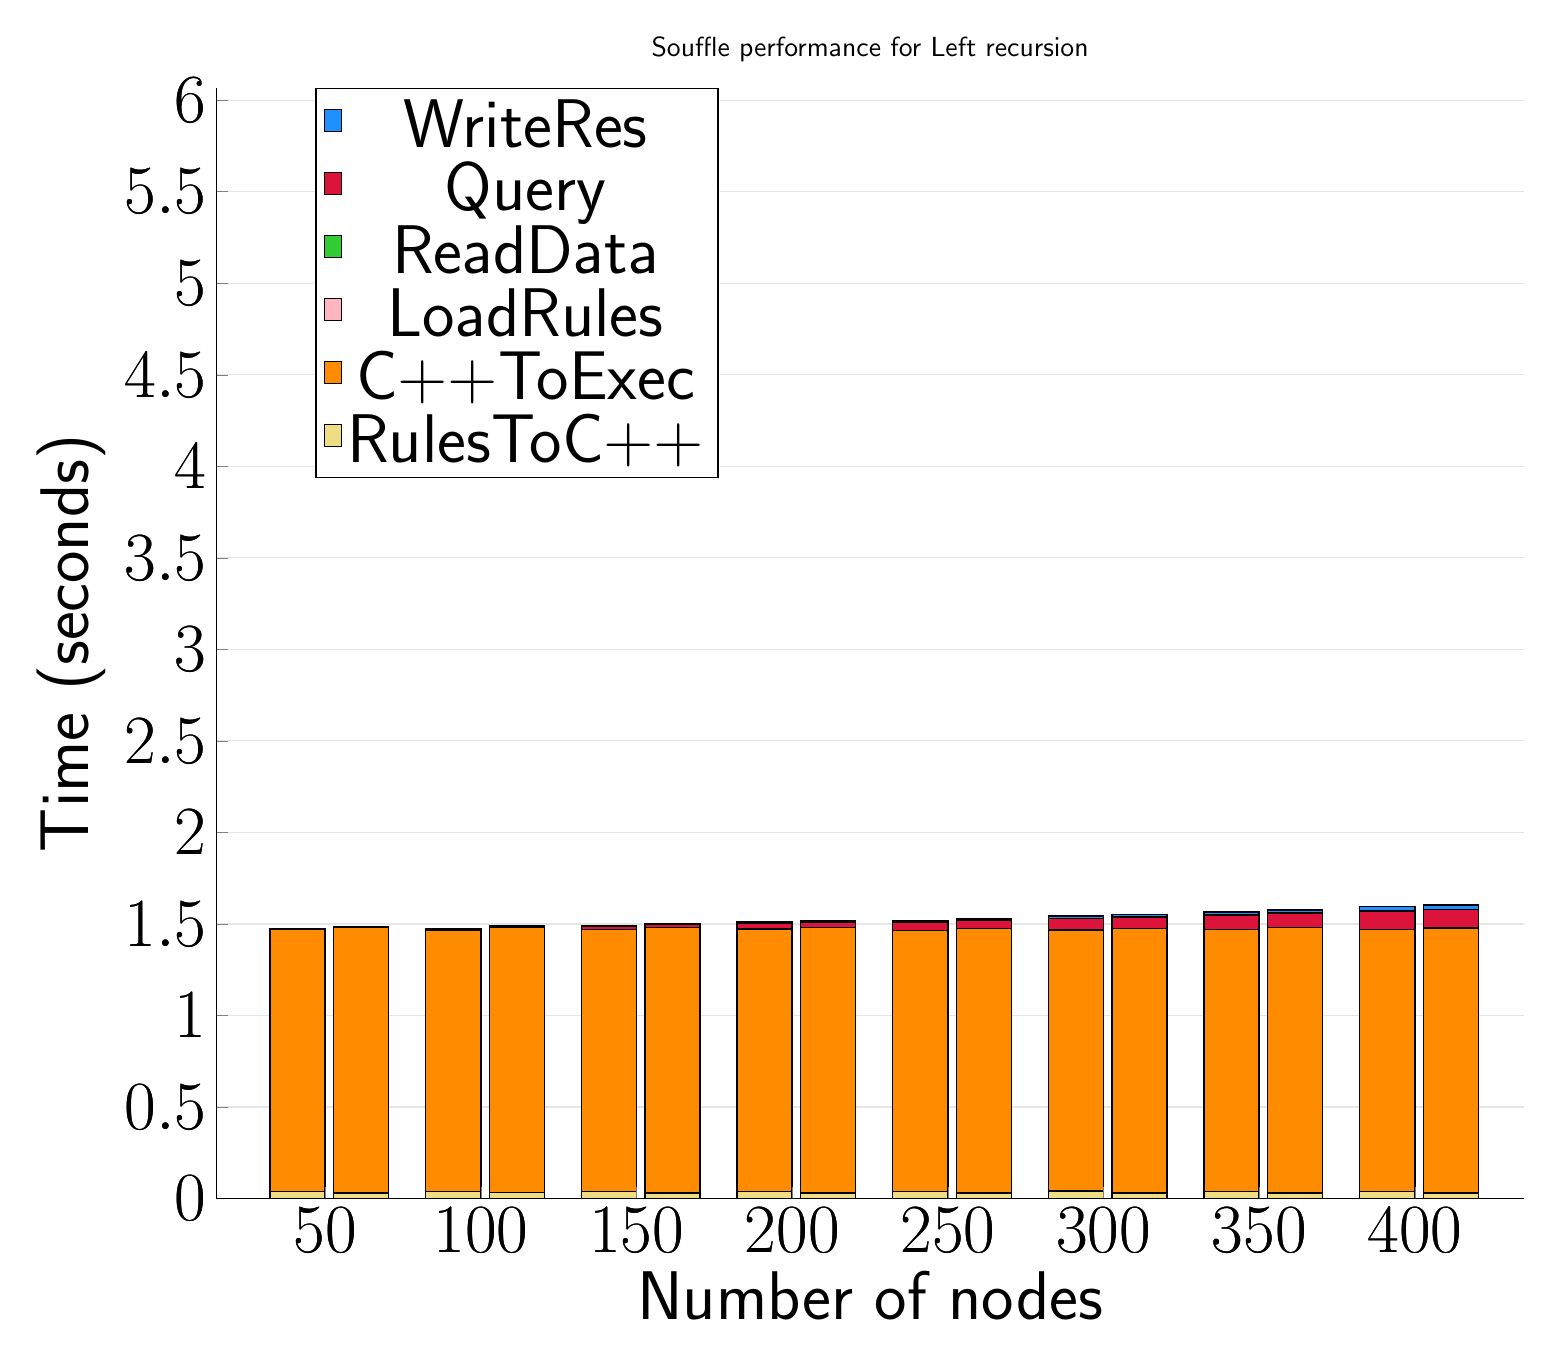
\begin{tikzpicture}
\begin{axis}[
   ybar stacked,
   title={Souffle performance for Left recursion},
   bar shift=-10pt,
   width=1.5\textwidth,
   bar width=0.7cm,
   ymajorgrids, tick align=inside,
   major grid style={draw=gray!20},
   xtick=data,
   ymin=0, ymax=6.067577,
   axis x line*=bottom,
   axis y line*=left,
   enlarge x limits=0.1,
   legend style={
       at={(0.23, 1)},
       anchor=north,
       legend columns=1,
       font=\Huge,
   },
   ylabel={Time (seconds)},
   xlabel={Number of nodes},
   label style={font=\Huge},
   tick label style={font=\Huge},
]
\addlegendimage{fill=DodgerBlue, draw=black, line width=0.2pt}
\addlegendentry{WriteRes}
\addlegendimage{fill=Crimson, draw=black, line width=0.2pt}
\addlegendentry{Query}
\addlegendimage{fill=LimeGreen, draw=black, line width=0.2pt}
\addlegendentry{ReadData}
\addlegendimage{fill=LightPink, draw=black, line width=0.2pt}
\addlegendentry{LoadRules}
\addlegendimage{fill=DarkOrange, draw=black, line width=0.2pt}
\addlegendentry{C++ToExec}
\addlegendimage{fill=LightGoldenrod, draw=black, line width=0.2pt}
\addlegendentry{RulesToC++}
\addplot +[fill=LightGoldenrod, draw=black, line width=0.5pt] coordinates {
    (50, 0.03899996280670166)
    (100, 0.03899998664855957)
    (150, 0.03900001049041748)
    (200, 0.039999985694885255)
    (250, 0.039999961853027344)
    (300, 0.04100000858306885)
    (350, 0.04000000953674317)
    (400, 0.040000081062316895)
};
\addplot +[fill=DarkOrange, draw=black, line width=0.5pt] coordinates {
    (50, 1.4330000162124634)
    (100, 1.4259999990463257)
    (150, 1.4299999952316285)
    (200, 1.4320000171661378)
    (250, 1.4240000247955322)
    (300, 1.4260000228881835)
    (350, 1.4299999952316285)
    (400, 1.428999948501587)
};
\addplot +[fill=LightPink, draw=black, line width=0.5pt] coordinates {
    (50, 9.45083e-05)
    (100, 0.00010146249999999999)
    (150, 8.711250000000001e-05)
    (200, 0.00012335010000000002)
    (250, 0.00012495)
    (300, 0.00012302490000000002)
    (350, 7.54209e-05)
    (400, 8.57335e-05)
};
\addplot +[fill=LimeGreen, draw=black, line width=0.5pt] coordinates {
    (50, 0.0003195375)
    (100, 0.00043805400000000006)
    (150, 0.0005247875)
    (200, 0.0006956709999999999)
    (250, 0.0007935083)
    (300, 0.0008886454)
    (350, 0.0009077295000000001)
    (400, 0.0010085292999999999)
};
\addplot +[fill=Crimson, draw=black, line width=0.5pt] coordinates {
    (50, 0.0016501869999999998)
    (100, 0.007935399999999999)
    (150, 0.01638466)
    (200, 0.03013297)
    (250, 0.04516944)
    (300, 0.06206594)
    (350, 0.07780325000000002)
    (400, 0.10126597)
};
\addplot +[fill=DodgerBlue, draw=black, line width=0.5pt] coordinates {
    (50, 0.0007944212000000001)
    (100, 0.002286825)
    (150, 0.004469588)
    (200, 0.007117754)
    (250, 0.009617391)
    (300, 0.012930819999999999)
    (350, 0.017428370000000002)
    (400, 0.022644110000000002)
};
\end{axis}
\begin{axis}[
   ybar stacked,
   bar shift=13pt,
   width=1.5\textwidth,
   bar width=0.7cm,
   ymajorgrids, tick align=inside,
   major grid style={draw=none},
   xtick=data,
   ymin=0, ymax=6.067577,
   axis x line*=none,
   axis y line*=none,
   enlarge x limits=0.1,
   label style={font=\Huge},
   tick label style={font=\Huge},
]
\addplot +[fill=LightGoldenrod, draw=black, line width=0.5pt] coordinates {
    (50, 0.030000000000000006)
    (100, 0.034)
    (150, 0.030000000000000006)
    (200, 0.030000000000000006)
    (250, 0.030000000000000006)
    (300, 0.030000000000000006)
    (350, 0.030000000000000006)
    (400, 0.030000000000000006)
};
\addplot +[fill=DarkOrange, draw=black, line width=0.5pt] coordinates {
    (50, 1.453)
    (100, 1.4479999999999997)
    (150, 1.4499999999999997)
    (200, 1.45)
    (250, 1.4449999999999998)
    (300, 1.4449999999999998)
    (350, 1.4509999999999998)
    (400, 1.4479999999999997)
};
\addplot +[fill=LightPink, draw=black, line width=0.5pt] coordinates {
    (50, 9.35e-05)
    (100, 0.00010080000000000002)
    (150, 8.66e-05)
    (200, 0.00012230000000000002)
    (250, 0.00012340000000000002)
    (300, 0.00012200000000000001)
    (350, 7.48e-05)
    (400, 8.53e-05)
};
\addplot +[fill=LimeGreen, draw=black, line width=0.5pt] coordinates {
    (50, 0.0003187)
    (100, 0.000437)
    (150, 0.0005239)
    (200, 0.0006938999999999999)
    (250, 0.0007925999999999999)
    (300, 0.0008845000000000001)
    (350, 0.0009070999999999999)
    (400, 0.0010073)
};
\addplot +[fill=Crimson, draw=black, line width=0.5pt] coordinates {
    (50, 0.0016471000000000003)
    (100, 0.0079314)
    (150, 0.0163472)
    (200, 0.0300908)
    (250, 0.0450924)
    (300, 0.061938400000000005)
    (350, 0.07762260000000001)
    (400, 0.1010922)
};
\addplot +[fill=DodgerBlue, draw=black, line width=0.5pt] coordinates {
    (50, 0.0007196)
    (100, 0.0022819)
    (150, 0.0043135)
    (200, 0.006930400000000001)
    (250, 0.009600599999999999)
    (300, 0.012846100000000003)
    (350, 0.017316900000000003)
    (400, 0.0226209)
};
\end{axis}
\end{tikzpicture}

\end{document}
